\documentclass[11pt]{standalone}
\usepackage{tikz}
\usetikzlibrary{fit,positioning}
\begin{document}
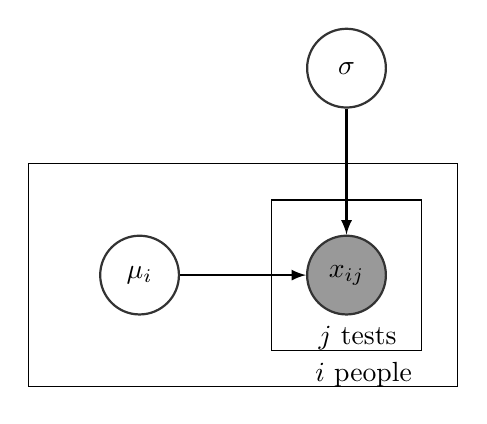
\begin{tikzpicture}
\tikzstyle{main}=[circle, minimum size = 10mm, thick, draw =black!80, node distance = 16mm]
\tikzstyle{connect}=[-latex, thick]
\tikzstyle{box}=[rectangle, draw=black!100]
  %\node[main, fill = white!100] (alpha) [label=below:$\alpha$] { };
  %\node[main] (mu) [right=of alpha,label=below:$\mu$] { };
\node[main] (mu) [] {$\mu_{i}$};
  \node[main, fill = black!40] (x) [right=of mu,label=below:] {$x_{ij}$};
  \node[main] (sigma) [above=of x] {$\sigma$ };
  %\path (alpha) edge [connect] (theta)
  % (theta) edge [connect] (z)
  \path (mu) edge [connect] (x)
		(sigma) edge [connect] (x);
  \node[rectangle, inner sep=0mm, fit= (x),label=below right:$j$ tests, xshift=-10mm] {};
  \node[rectangle, inner sep=4.4mm,draw=black!100, fit= (x)] {};
  \node[rectangle, inner sep=4.6mm, fit= (x),label=below right:$i$ people, xshift=-15mm] {};
  \node[rectangle, inner sep=9mm, draw=black!100, fit = (mu) (x)] {};
\end{tikzpicture}
\end{document}
%note - compiled with pdflatex